\documentclass[10pt,journal,cspaper,compsoc]{IEEEtran}
%
\ifCLASSINFOpdf
  \usepackage[pdftex]{graphicx}
  \DeclareGraphicsExtensions{.pdf,.jpeg,.png}
\else
  \usepackage[dvips]{graphicx}
\fi

\usepackage{comment}
\usepackage{listings}
\usepackage{pgf}
\usepackage{amsmath}
\usepackage{subfigure}
\usepackage{tikz}
\usepackage{tikz-qtree}
\usetikzlibrary{arrows,automata}

\lstset{
  basicstyle = \ttfamily\scriptsize\color{black},%\bfseries
  keywordstyle = \color{red},%\bfseries
  keywordstyle = [2]\ttfamily\color{black},
  frame = single,
  captionpos=b,
  frame=single,
  tabsize=2,
  xleftmargin=15pt,
  numbers=left
}

\definecolor{darkgreen}{rgb}{0,0.7,0}

\newif\ifdraft
\drafttrue
%\draftfalse
\ifdraft
 \newcommand{\katznote}[1]{ {\textcolor{blue}    { ***Dan:      #1 }}}
 \newcommand{\ketanote}[1]{{\textcolor{orange}    { ***Ketan:      #1 }}}
 \newcommand{\note}[1]{ {\textcolor{red}    {\bf #1 }}}
\else
 \newcommand{\katznote}[1]{}
 \newcommand{\ketanote}[1]{}
 \newcommand{\note}[1]{}
\fi
% correct bad hyphenation here
\hyphenation{op-tical net-works semi-conduc-tor}

\setlength\parindent{0pt}

\begin{document}
% can use linebreaks \\ within to get better formatting as desired
\title{Evaluating Storage Systems for Scientific Data in the Cloud}
% \title{Evaluation of global-scale programming and data storage techniques
%        in cloud computing}

\author{\IEEEauthorblockN{Ketan Maheshwari\IEEEauthorrefmark{1},
Justin M. Wozniak\IEEEauthorrefmark{1},
Hao Yang\IEEEauthorrefmark{2},\\
Daniel S. Katz\IEEEauthorrefmark{3},
Matei Ripeanu\IEEEauthorrefmark{2},
Victor Zavala\IEEEauthorrefmark{3},
Michael Wilde\IEEEauthorrefmark{1}\IEEEauthorrefmark{3}\\
\IEEEauthorblockA{
\IEEEauthorrefmark{1}MCS Division, Argonne National Laboratory, Argonne, IL 60439}\\
\IEEEauthorrefmark{2}Department of Electrical and Computer Engineering,  University of British Columbia\\
\IEEEauthorrefmark{3}Computation Institute,  University of Chicago \& Argonne National Laboratory}
}

\maketitle
\begin{abstract}
Infrastructure-as-a-Service (IaaS) clouds are an appealing resource for
scientific computing. 
%
However, the bare-bones presentation of raw Linux virtual machines leaves much
to the application developer.
%
For many cloud applications, effective data handling is critical to efficient
application execution.
%
This paper investigates the capabilities of a variety of POSIX-accessible
distributed storage systems to manage data access patterns resulting from
workflow application executions in the cloud.
%
We leverage the expressivity of the Swift parallel scripting framework to
benchmark the performance of a number of storage systems using synthetic
workloads and three real-world applications. We characterize two representative
commercial storage systems (Amazon S3 and HDFS, respectively) and two
emerging research-based storage systems (Chirp/Parrot and MosaStore). We find
the use of aggregated node-local resources effective and economical compared
with remotely located S3 storage. Our experiments show that applications run at
scale with MosaStore show up to 30\% improvement in makespan time compared with
those run with S3.
%
We also find that storage-system driven application deployments in the cloud
results in better runtime performance compared with an on-demand data-staging
driven approach.

%TODO: Summarize conclusions/lessons
%
\end{abstract}
\begin{IEEEkeywords}
HPC, parallel computing, cloud, storage systems
\end{IEEEkeywords}

\IEEEpeerreviewmaketitle

\section{Introduction}
%TODO: Improve introduction, we're not talking about exascale
%TODO: Add a clear plan for the paper: a hierarchical diagram of things we are addressing in the paper. And things we are not.

Clouds are poised to become a key platform for data-intensive distributed 
computing~\cite{cloudreq}. Through virtualization, clouds offer full ownership
of a flexible and customizable infrastructure. The Magellan
initiative on cloud usability and data management~\cite{magellan1} examined the
cloud model for scientific applications. One of the challenges identified in
its final report~\cite{magellan2} was developing appropriate application
programming models that enhance the capabilities of the existing MapReduce
model:

\begin{quote}
Tools to simplify using cloud environments ... and enhancements to
MapReduce models to better fit scientific data and workflows [are needed] for
scientific applications. The current tools often require significant porting
effort, do not provide bindings for popular scientific programming languages,
and are not optimized for the structured data formats often used in large-scale
simulations and experiments. 
\end{quote}

More recently, a survey conducted by XSEDE~\cite{xsede:cloudsurvey} indicated
the increasing cloud adoption in the scientific community. One of the
challenges reported by a majority of the users interviewed was the difficulty
and cost associated with managing data. Furthermore, the survey indicated that
many users (27\%) use the costly object store services such as S3 for
application data management. On the other hand, experience using and comparing
clouds with traditional high-performance computing (HPC)
environments~\cite{marathe, cloudvcluster} sheds light on the advantages of the
cloud:

\begin{itemize}
\item The virtualized environment of the cloud eliminates the queue waiting times
often dominating application turnaround times in shared clusters.
The queue wait times have been replaced by the time it takes virtual machines (VMs) to become
available. (Our past experiments show that this is generally under one minute
on popular clouds such as EC2 and is constant regardless of the requested
number of VMs~\cite{swift13}).

\item Administrator-level access to instances in the cloud gives more control over
resources, aiding in a range of user activities, such as installation and
upgrade of software tools, and in customization of network policies, such as
firewalls, without jeopardizing the system security.

\item Clouds offer an economically affordable solution under certain cost models. 
\end{itemize}

Despite these advantages, however, there is a lack of suitable techniques and
tools to manage application data effectively and economically on distributed
cloud resources.

This paper explores the coupling of a programming model suitable for a popular
application class, namely, many-task computing, with various storage
systems suitable for the cloud. Specifically, we use the Swift
parallel scripting framework with virtual storage and file management systems
(collectively, storage systems) in cloud computing environments and
assess their impact on application performance and overall usability. To better
understand the practicalities of these systems, we benchmark the overall
performance of the coupled system using both synthetic workloads and real-world
applications.

This paper makes contributions over multiple axes: 

\begin{enumerate}
\item Platform characterization: it sheds light on the network characteristics
    between Amazon EC2 cloud provisioning regions not generally taken into
    account while building computational models.

\item Storage system performance characterization: it benchmarks the
performance of various storage systems with respect to core data
access patterns. 

\item Application porting to the cloud: It demonstrates execution of real-world
applications on the cloud via a parallel scripting programming approach under
two distinct data management models. More important, it helps in
understanding the tradeoffs resulting from the choice of the storage
system to support workflow applications. 

\item Guidelines for toolkit evolution for clouds: It makes a case for
improved usability of the cloud computing model using tools well adapted to
traditional tightly coupled systems such as HPC clusters. 
\end{enumerate}

% ===== 
\usetikzlibrary{arrows,shapes,positioning,shadows,trees}

\tikzset{
  basic/.style  = {draw, text width=2cm, drop shadow, font=\sffamily, rectangle},
  root/.style   = {basic, rounded corners=2pt, thin, align=center,
                   fill=green!30},
  level 2/.style = {basic, rounded corners=6pt, thin,align=center, fill=green!60,
                   text width=8em},
  level 3/.style = {basic, thin, align=left, fill=pink!60, text width=6em}
}
\begin{figure*}
\centering
\begin{tikzpicture}[
  level 1/.style={sibling distance=40mm},
  edge from parent/.style={->,draw},
  >=latex]

% root of the the initial tree, level 1
\node[root] {Cloud Resources}
% The first level, as children of the initial tree
  child {node[level 2] (c1) {Computation}}
  child {node[level 2] (c2) {Storage}}
  child {node[level 2] (c3) {Network}};

% The second level, relatively positioned nodes
\begin{scope}[every node/.style={level 3}]
\node [below of = c1, xshift=15pt] (c11) {CPU speeds};
\node [below of = c11] (c12) {CPU count};
\node [below of = c12] (c13) {CPU kind};

\node [below of = c2, xshift=15pt] (c21) {On node};
\node [below of = c21] (c22) {Block Device};
\node [below of = c22] (c23) {Remote Online};
\node [below of = c23] (c24) {Remote Offline};

\node [below of = c3, xshift=15pt] (c31) {Bandwidth};
\node [below of = c31] (c32) {Latencies};
%\node [below of = c32] (c33) {Resizing tips};
%\node [below of = c33] (c34) {Shortening};
%\node [below of = c34] (c35) {Bending};
\end{scope}

% lines from each level 1 node to every one of its "children"
\foreach \value in {1,2,3}
  \draw[->] (c1.195) |- (c1\value.west);

\foreach \value in {1,...,4}
  \draw[->] (c2.195) |- (c2\value.west);

\foreach \value in {1,...,2}
  \draw[->] (c3.195) |- (c3\value.west);
\end{tikzpicture}
\caption{Scope of current research}
\label{fig:scope}
\end{figure*}
% ===== 

While we touch upon the subject of cost, we consider it outside of the scope of
this paper and do not analyze it in any detail. The rest of this paper is
structured as follows.  Network characteristics of global EC2 cloud are
analyzed in Section~\ref{sec:understanding}. Virtual storage solutions used in
the current study are described in Section~\ref{sec:storage}. The Swift
parallel scripting framework is briefly discussed in Section~\ref{sec:swift}.
Our experiment setup for cloud related experiments is described in
Section~\ref{sec:expsetup}.  Section~\ref{sec:perf} evaluates the performance
of storage solutions for common workflow data access patterns.  We discuss
three use-case applications in Section~\ref{sec:app} and present evaluation in
Section~\ref{sec:appresults}. Related work is discussed in
Section~\ref{sec:related}. We present concluding remarks and future work in
Section~\ref{sec:concl}.

\section{The Nature of the Cloud}\label{sec:understanding}
Cloud vendors often do not reveal the true nature of the underlying fabric
behind the virtualized resources. Clouds such as Amazon EC2 can have a global
span. Users have limited information about the topology, network, and hardware
capabilities. Consequently, one must explore available clues to gauge the
nature of cloud environments and the best solutions for efficiently using
resources. 

Figures~\ref{fig_bw} and \ref{fig_lat} present the bandwidth and latency,
respectively, between instances from all eight available regions of Amazon EC2
cloud. Depending on the platform and application requirements, questions that
must be answered include the following: What are the network capacity and
latency between cloud instances at the zone, region, and global level? What is
the expected time to completion given a fixed number of resources in a given
set of regions? What are the tradeoffs between storage and network performance
that inform advanced data management solution?  Which additional region is best
to draw resources from, once the resource allocation limits have been reached
in a given region?

The results obtained in figures~\ref{fig_bw} and~\ref{fig_lat} are significant
for the consumers of cloud infrastructures that are deployed over global
networks. While the infrastructure is presented to the user as a single virtual
platform, the expected performance of application will vary wildly dependent
upon the factors beyond a users control. This not only risks applications
performance but also increases the user costs of using the infrastructure.

Performance of distributed applications significantly rely upon the bandwidth
and latencies of the underlying infrastructure~\cite{latency}. Storage systems
such as the ones discussed in this paper circumvent these issues to some extent
by implementing efficient caching, replication, and prediction mechanisms.

\begin{figure}[htb]
\begin{center}
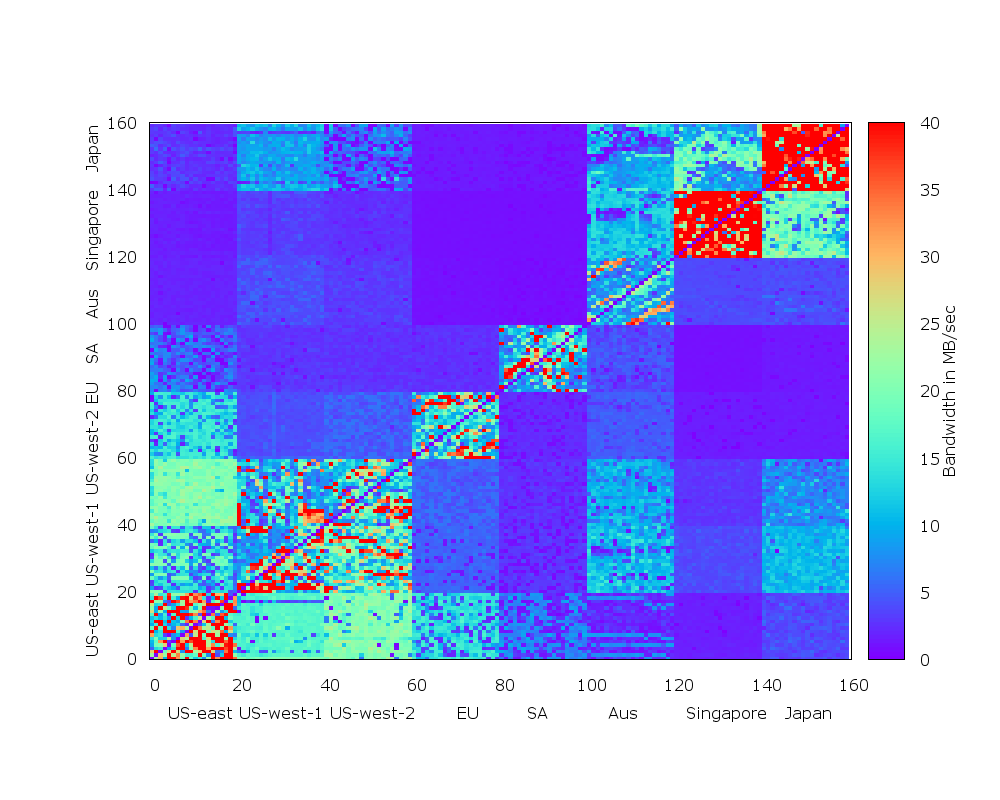
\includegraphics[width=\linewidth]{plots/bwheatmap.png}
%\label{fig_snap}
\caption{Heatmap of network bandwidths between instances of global Amazon EC2 cloud environment.
\label{fig_bw}
}
\end{center}
\end{figure}
%
\begin{figure}[htb]
\begin{center}
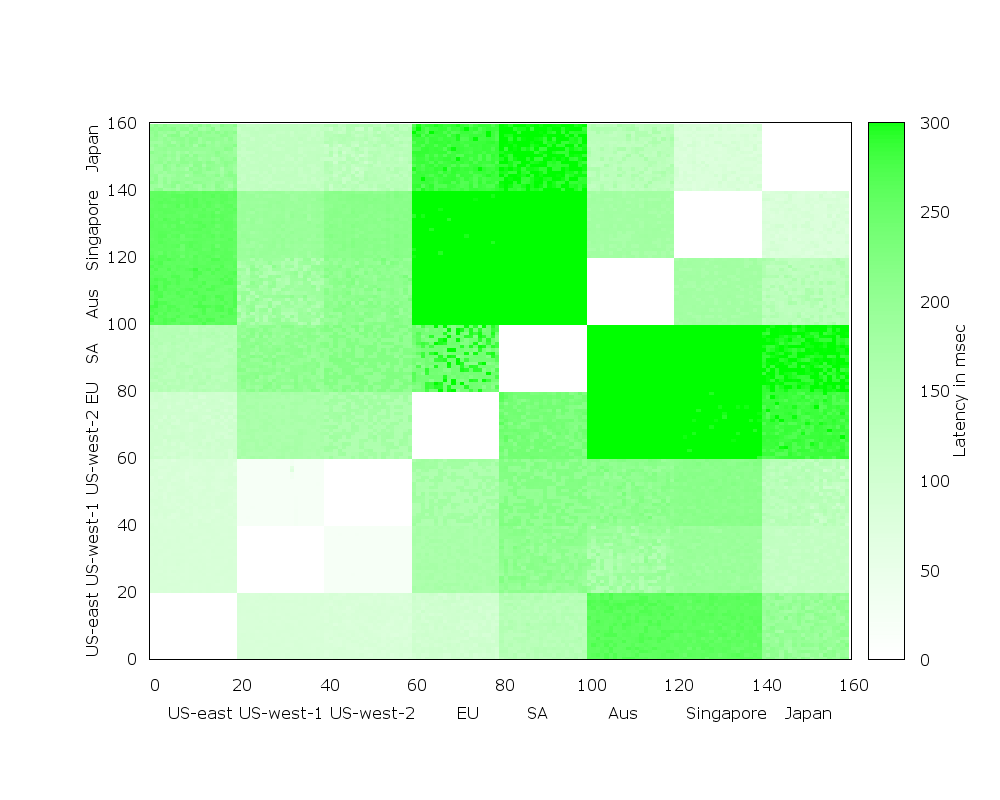
\includegraphics[width=\linewidth]{plots/latheatmap.png}
%\label{fig_snap}
\caption{Heatmap of network latencies between instances of global Amazon EC2 cloud environment.
\label{fig_lat}
}
\end{center}
\end{figure}

\section{Storage Systems}\label{sec:storage}

%\begin{figure*}[htb]
%\begin{center}
%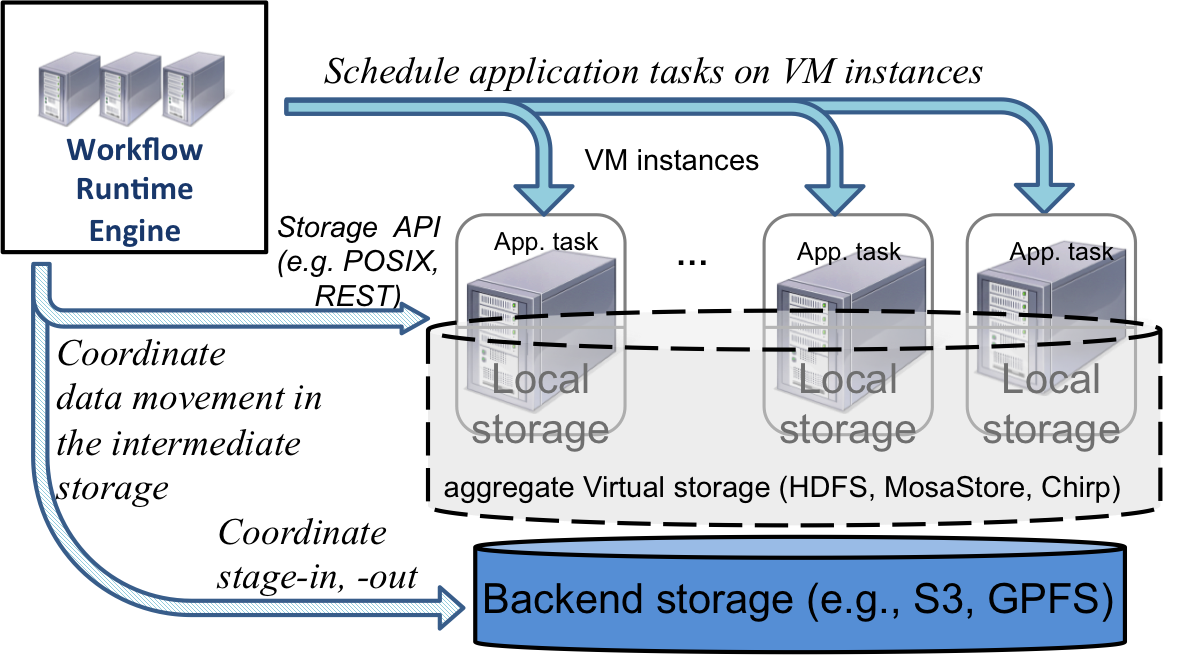
\includegraphics[width=4in]{figures/storage.png}
%\caption{An overview of workflow systems interaction with storage solutions.
%\label{fig_storage}
%}
%\end{center}
%\end{figure*}

Computing via workflows that assemble complex processing stages using existing
components as their building blocks is an established method in the science
domain. A popular approach to support these workflows is the many-task
approach, in which the workflow processes communicate through intermediary
files stored on a shared file-system.

On clouds, however, the backend data storage system can become a bottleneck
when supporting I/O-intensive workflows~\cite{works-ame}. Hence, an
increasingly popular way to support workflow applications is to harness some of
the resources allocated by the cloud, particularly node-local storage, and
assemble a scratch storage space to store the intermediary data used to
communicate among workflow tasks. In this scenario,
the workflow scheduler is in charge of staging the application data into the
intermediate space and staging out the results as needed. The details of
workflow enactment depends on the precise data access semantics and API offered
by this intermediate space. At one end of the spectrum are intermediate storage
systems that offer a shared file-system with complete POSIX API support (e.g.,
MosaStore~\cite{MosaStore_2010, MosaStore_2012}, and
Chirp/Parrot~\cite{chirp}). Whereas, at the other end of the spectrum are two
overlapping solutions: (1) solutions that offer a custom API, possibly
specialized for classes of applications (e.g., the Hadoop File System - HDFS);
and, (2) solutions that do not offer a shared name and storage space and leave
explicit data movement between independent storage nodes and space management
to be handled by the workflow scheduler. Apart from performance, an additional
benefit from using the storage systems is lower cost: most cloud billing
systems do not invoice separately the instance-local storage space/traffic;
thus, deploying and using an intermediate storage space comes at zero cost (as
opposed to using the backend storage where both space and traffic are generally
billed). 
%
%We study the performance of S3, the backend storage system available on the
%Amazon cloud, with the performance of a set of intermediate storage systems
%that offer different tradeoffs in terms of usability and configurability.  In
%particular we look at HDFS, MosaStore, and Chirp/Parrot and deploy them to
%aggregate the node-local storage resources over the VM instances allocated to
%the application.
\subsection{Amazon S3} 
Amazon S3~\cite{s3_web} is the storage service provided by Amazon. Its full
design and architecture have not been made public; however, an important
building block is the Dynamo~\cite{dynamo} key-value store. S3 was not designed
to be a file system and is not POSIX-compatible.  It acts as a large-scale
datastore and backup service for cloud-based applications.
S3 is preconfigured, albeit at a cost charged by
Amazon. It has a simple two-level namespace: buckets (with unique names in the
global namespace) and objects (the data stored within the buckets). It provides
durability, availability, and relatively fast access. These characteristics
make S3 an ideal service for applications requiring backup and archiving (e.g.,
the Smart Grid State Estimation application ~\cite{maheshwari-lim-etal:2013}).
Third-party interfaces such as S3FS~\cite{s3fs_web} provide access to S3
service as mountable file systems with a subset of common file operations. S3FS
also implements a simple, local node caching mechanism to improve performance
over that of raw S3 access.

\subsection{Hadoop Distributed File System}
The Hadoop Distributed File System (HDFS) is a high-throughput file system
designed to store and process large amounts of data stored on cheap,
shared-nothing clusters of commodity machines. HDFS aggregates the disk space
of the distributed nodes on which it is installed and provides a unified
storage view of the aggregated space. A block of data (usually 64 MB) is the
unit of management for load balancing, physical data movement, replication, and
fault tolerance. Data movement is governed via ``streaming" access modes,
implying its suitability for record-level manipulation on datasets. Metadata
and file namespace on an HDFS cluster are managed by a ``NameNode" process. The
actual data blocks are managed by the ``DataNode" processes running on each
compute node of a cluster. 

\subsection{MosaStore}
MosaStore is a low-overhead, user-level distributed storage system based on
FUSE~\cite{fuse_web}. MosaStore can be deployed to aggregate the storage space
of compute nodes to an application and offered it as a shared POSIX-compatible
storage system.  MosaStore is workflow—optimized in that it supports various
data placement optimizations designed specifically for workflow applications.
Its key attributes are: (1) The POSIX API makes integration with applications
trivial; (2) Files are striped across multiple nodes. This is a useful feature
if nodes do not have disks and if RAM disks with inherently limited space need
to be aggregated; and (3) Support is provided for cross-layer optimizations
that enable the storage system to expose details of the stored data (e.g., data
location, replication level) to an application or workflow. 

\subsection{Chirp/Parrot}
Chirp~\cite{chirp} is a user-level storage system that provides a virtualized,
unified view of data over multiple real file systems (e.g., over file systems
deployed over independent clusters). Deploying Chirp does not require kernel
changes or special access privileges (admittedly, not a key issue when
deploying on cloud, but often a major adoption barrier when using large, shared
clusters). Chirp servers consist of directory servers (containing only the
directory hierarchy of the Chirp name\-space) and data servers (containing the
actual files). The files are not striped across multiple nodes. Parrot is an
interceptor layer that traps the application's POSIX file system calls and
redirects them to Chirp. A combination of Parrot and Chirp can thus provide a
POSIX-accessible storage environment with files distributed across multiple
native file systems.

\subsection{Summary of Storage Systems Features}
In this section, we summarize the operations of the storage systems, showing
the common abstractions and working mechanisms. Storage systems can be seen as
having three components (though in some cases these components are minimal):

\begin{enumerate}
\item On the client side (where the client application runs), a component
    that enables the application to access the data.  This can be as complex as
    FUSE-based implementation in MosaStore (or S3 access through S3FS),
    Java APIs for HDFS, or an ability to deal with file
    management and transfers ( e.g., Parrot for Chirp).

\item On the storage side, the basic native storage (block or chunk level) and a
    component that exposes it to the rest of the system, and signals that the
    component is active to enable discovering failures, decision system to
    replication, liveliness etc (e.g. Mosastore's benefactor component). 

\item A management component that keeps track of functionalities involving
    striping, space management, garbage collection, data placement, etc.  Not
    all systems have all these; some (e.g., Chirp) leave the applications to
    manage these functionalities by themselves.
\end{enumerate}

\section{Swift}\label{sec:swift}
We use the Swift parallel scripting framework to express application flow and
orchestrate tasks on clouds. 

Swift~\cite{Swift_2011} is an implicitly concurrent programming language
originally designed to express workflows consisting of large numbers of
scientific application invocations on multiple diverse resources. Swift
separates application workflow logic from runtime configuration, allowing for a
highly flexible development model. Swift can invoke application binaries on
distributed resources, similar to ordinary command-line invocations, rendering
better binding with application execution environment without extra coding
required from the user. Swift/K is a parallel scripting framework for
distributed application programming. It supports explicit data movement via
protocols such as FTP, scp, and TCP. A pilot-job abstraction is supported via
its coasters implementation~\cite{Coasters_UCC_2011}. The Swift/T engine (T
stands for Turbine, a distributed engine)~\cite{fi:2013} distributes the load
of processing Swift workflow logic across multiple sites. This enables
extremely scalable workflow logic processing and task management. 

\section{Experiment Setup}\label{sec:expsetup}
We prepared a Linux image with the tools and software installation and required
security and communication tuning. FUSE was installed and enabled as a kernel
module.  The Chirp server was installed on each of the cloud instances' EBS
device.  Read/write operations were performed on randomly chosen Chirp servers
via explicit calls to Parrot. For HDFS, a default setup mimicking that of
Hadoop applications was used. An instance was chosen as a NameNode, whereas the
rest of the instances were designated as DataNodes with storage space formatted
over the EBS device. One of the DataNodes served as a secondary NameNode. For
MosaStore, one instance was designated as the manager node whereas the rest of
the instances were the benefactor nodes. The application binaries and library
dependencies were installed on the image.  Application input data was loaded on
the storage systems or on local EBS storage as required. In all experiments,
instances drawn from the same prepared image were size ``m1.large", consisting
of two cores and 8~GB memory each.

\section{Raw performance evaluation}\label{sec:perf}
The fundamental I/O patterns in workflows involve successive reads and writes
occurring concurrently on file systems for interdependent and independent
tasks. In this section we explore the common I/O patterns of workflow
applications and look into the performance on underlying storage systems. In order to
ensure uniformity in data movement, as seen in Section~\ref{sec:understanding}
the instances are drawn from a single region for the experiments described in
this section.

Performance benchmarks for parallel reads of data of varying sizes from the
underlying storage systems are shown in figure~\ref{fig:par-rd-bench}. The data
is read from the respective storage system into the local file system, EBS
devices in the case of Amazon cloud.

\begin{figure}[htb]
\begin{center}
%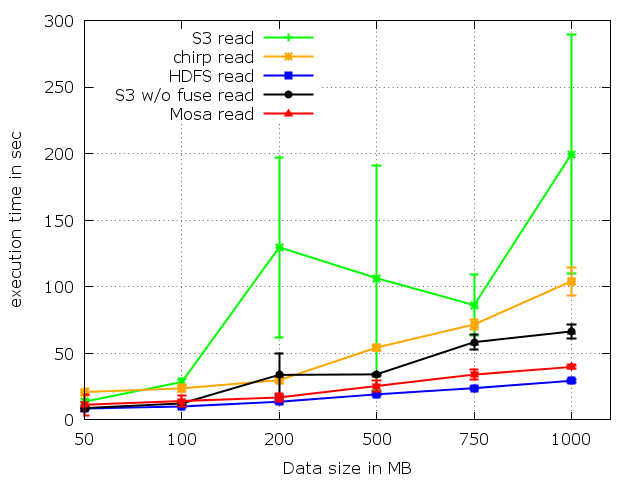
\includegraphics[width=\linewidth]{plots/par-read-benchmark.png}
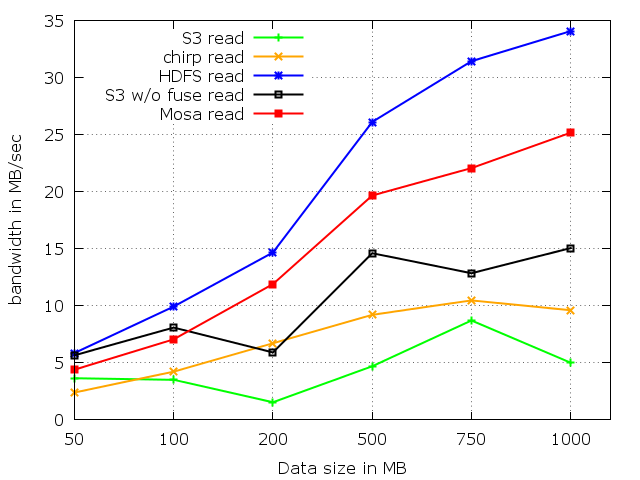
\includegraphics[width=\linewidth]{plots/par-read-bw.png}
\caption{Performance benchmark of storage systems on Amazon cloud:
concurrent reads of 40 files with varying size across 40 Amazon nodes.
\label{fig:par-rd-bench} }
\end{center}
\end{figure}

Performance benchmarks for parallel writes of data of varying sizes to the
underlying storage systems are shown in figure~\ref{fig:par-wr-bench}. The data
is written to the storage system from the local file system.

\begin{figure}[htb]
\begin{center}
%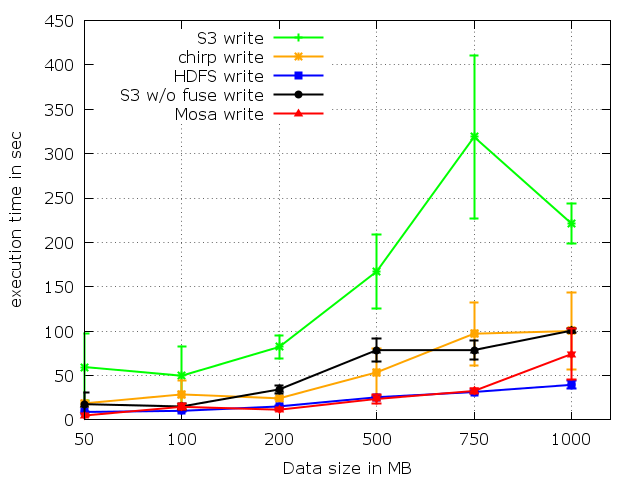
\includegraphics[width=\linewidth]{plots/par-write-benchmark.png}
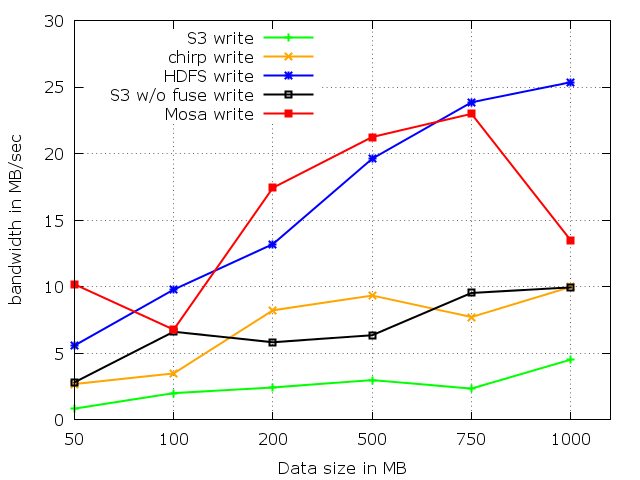
\includegraphics[width=\linewidth]{plots/par-write-bw.png}
\caption{Performance benchmark of virtual storage systems on Amazon cloud:
concurrent writes of 40 files with varying size across 40 Amazon nodes
\label{fig:par-wr-bench} }
\end{center}
\end{figure}

%\subsection{Read After Write}
In read-after-write (RAW)
pattern, shown in figure~\ref{fig:raw}, data is read from the storage
immediately after being written to it. 
%
\begin{figure*}[htb]
\begin{center}
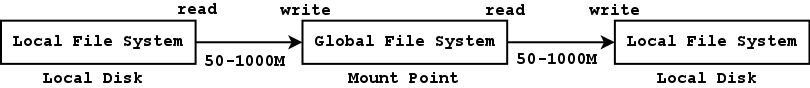
\includegraphics[width=13cm]{figures/raw.png}
\caption{Read-after-write data access pattern: data is read immediately after being written to a global storage system mount point.
\label{fig:raw}
}
\end{center}
\end{figure*}
%
Shown in figure~\ref{fig:raw_perf} are the performance measurement plots for the RAW pattern on varying data sizes.
%
\begin{figure}[htb]
\begin{center}
%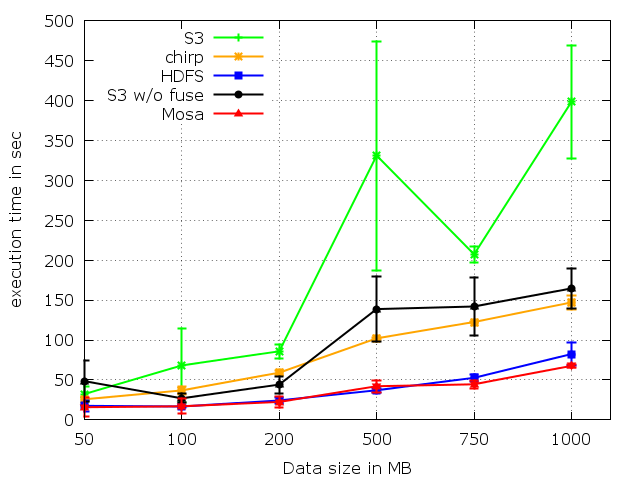
\includegraphics[width=\linewidth]{plots/RAW-benchmark.png}
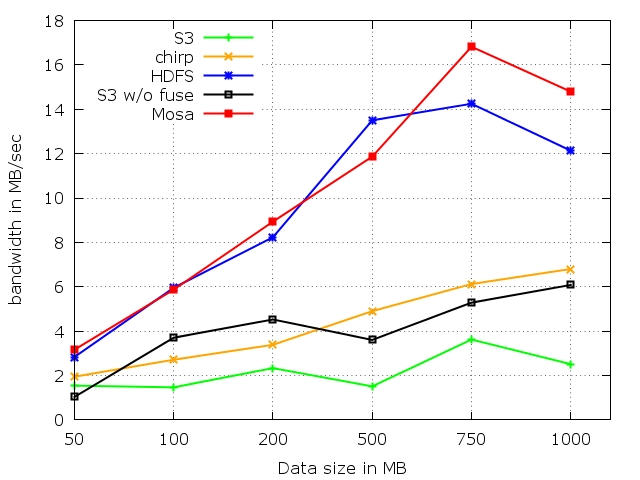
\includegraphics[width=\linewidth]{plots/RAW-bw.png}
\caption{Performance benchmarks for 40 concurrent read-after-writes on 40 EC2 nodes.
\label{fig:raw_perf}
}
\end{center}
\end{figure}
%
From the performance benchmarking plots, we see a trend of high variability on
the remotely located S3 system and a more consistent behavior from the storage
systems installed over local space. we see  consistently better bandwidths for
HDFS and MosaStore systems except at the 1000~MB datasizes. One of the most
common data access pattern in many-task workflow applications is concurrent
reads and writes. We see that MosaStore shows better read-after-write
performance beyond 500MB~(fig~\ref{fig:raw_perf}). Consequently, we chose
MosaStore for node-local aggregated storage for application measurements.

\section{Synthetic Workflow Application Performance Evaluation}


\subsection{calibration}

\section{Application Overview}\label{sec:app}
%\katznote{an intro sentence/paragraph is needed here}
In this section we describe three real-world applications and their
implementation using the virtual storage systems coupled with Swift. 

\subsection{Power Locational Marginal Price Simulation (LMPS)}
Optimal power flow studies are crucial in understanding the flow and price
patterns in electricity under different demand and network conditions. A big
computational challenge arising in power grid analysis is that simulations need
to be run at high time resolutions in order to capture effects occurring at
multiple time scales. The power flow simulation application under study
analyzes historical conditions in the Illinois grid to simulate instant power
prices on an hourly basis. The application runs linear programming solvers
invoked via an AMPL (A Mathematical Programming Language) model
representation and collects flow, generation, and price data with attached
geographical coordinates. A typical application consists of running the model
in 8,760 independent executions corresponding to each hour of the year.
%Each
%application task execution ranges from 11.7 to 84.5 seconds as
%shown in the application tasks time distribution graph in
%figure~\ref{fig:apptimes}. 
%A complete Swift/T representation of the application
%is shown in Listing~\ref{lst:lmps}.  
%
%\begin{lstlisting}[caption=Swift/T code for the power grid pricing simulation application, label=lst:lmps][ht]
%app (file amplout) runampl
% (file model, file bundle, int idx){
%  "runampl.sh" @model @bundle idx @amplout;
%}
%main{
%  file model=input_file("edrevised.run");
%  file bundle=input_file("bundle.tgz");
%  file amplout[];
%  int num-hrs=8760; //365 X 24
%  foreach i in [1:num-hrs]{
%    file t<sprintf("amplout-%i.tgz", i)>=
%         runampl (model, bundle, i);
%    amplout[i] = t;
%  }
%}
%\end{lstlisting}
%
%The ``app" declaration declares the application call prototype used
%to call an external application executable ``runampl.sh" which will be called
%with the parameters as command line arguments. The execution starts in ``main",
%where input and output files are declared, followed by a call to
%the application prototype in a parallel foreach loop with a range of 1 to 8,760.

\subsection{Parallel Blast}
Blast is one of the most prevalent applications used on clouds. A protein
alignment search tool, Blast performs searches from protein databases. Parallel
Blast workflow adds two additional steps to the basic Blast application. First,
a splitter splits the protein database into multiple fragments on which the
traditional Blast can be run. Second, the resulting search results from each of
the blast are merged using a blastmerge step. The application flow and its
interaction with underlying storage system is shown in figure~\ref{fig_blast}.
In this study we use a reduced `nr' nucleotide database with 1.5 million
entries. The splitter splits this database into 300 fragments resulting in a
total of 602 application calls.

\begin{figure}[htb]
\begin{center}
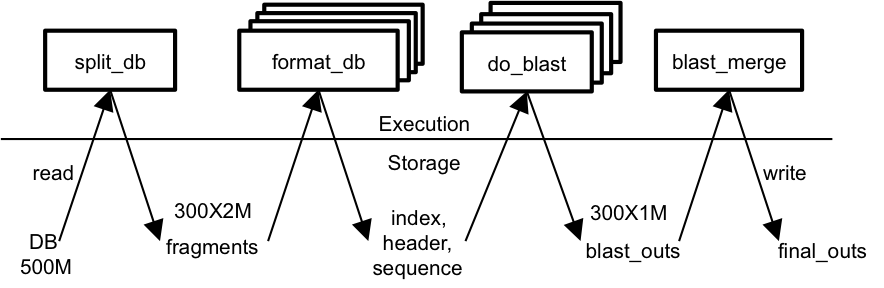
\includegraphics[width=\linewidth]{figures/blast.png}
%\label{fig_snap}
\caption{Blast application and its interaction with storage systems. 
\label{fig_blast}
}
\end{center}
\end{figure}

\begin{figure}[htb]
\begin{center}
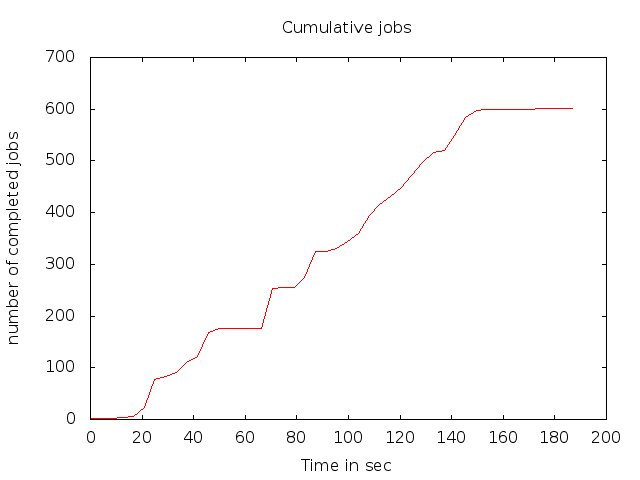
\includegraphics[width=\linewidth]{plots/blast_40i_80c.png}
%\label{fig_snap}
\caption{Blast application cumulative task execution plot with Swift/K data staging. A total of 602 tasks were run on 40 cloud instances. 
\label{fig_blast_k}
}
\end{center}
\end{figure}

\begin{figure}[htb]
\begin{center}
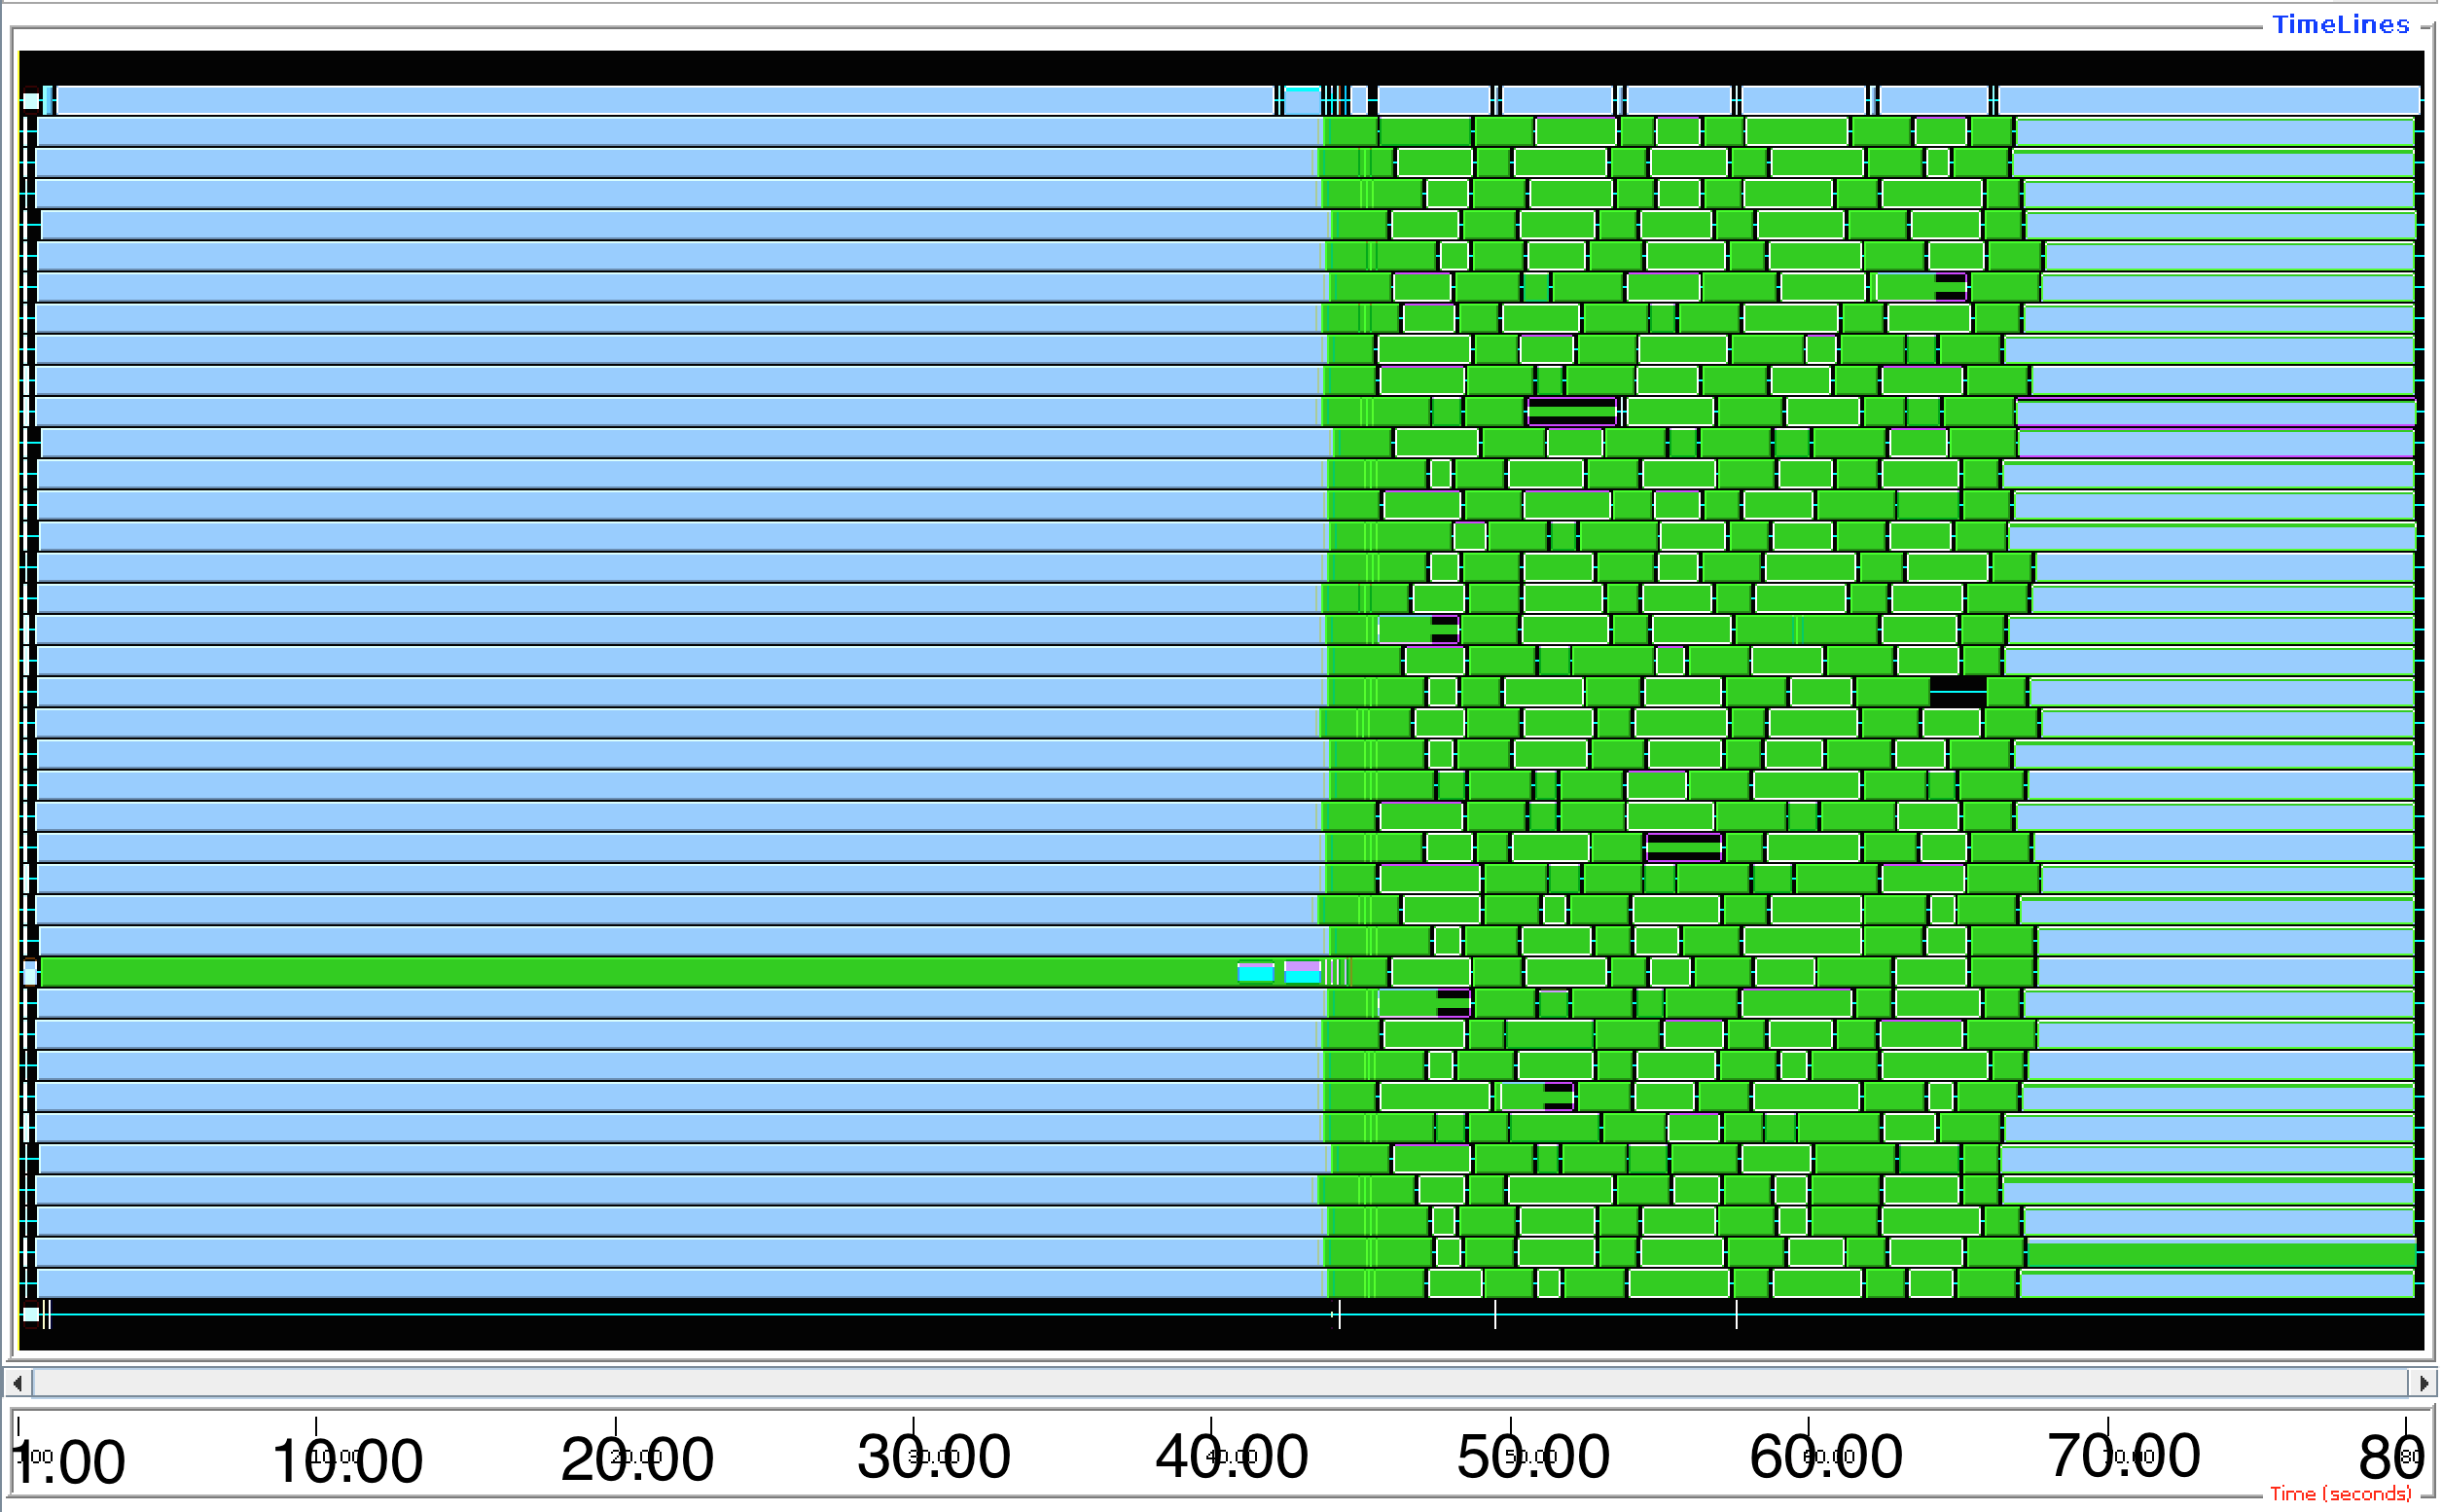
\includegraphics[width=\linewidth]{plots/blast_timeline_40i_80c_new.png}
%\label{fig_snap}
\caption{Blast application execution trace with Swift/T and MosaStore data
staging; A total of 602 tasks run on 40 cloud instances. The light blue
bars indicate worker-coordination wait; green bars indicate the
executions.
\label{fig_blast_t}
}
\end{center}
\end{figure}

\subsection{EnergyPlus}
%Application description
The EnergyPlus application is a suite of energy analysis and thermal load
simulation programs~\cite{eplus}. The application takes into account the local
historical climate and materials properties data to calculate an estimated
energy consumption of a building. The application can
take an ensemble of parameters such as orientation and height and compute
distinct sets of energy requirements. In our study, we vary the orientation of
a building located in Chicago between 10 and 100 degrees at a step size of 10,
combined with building height between 9 and 30 meters, resulting in 210
permutations. A postprocessing step after each EnergyPlus call converts the
resulting data into a summarized json format. The total number of tasks in this
application is 420 (figure~\ref{fig_eplus}).

\begin{figure}[htb]
\begin{center}
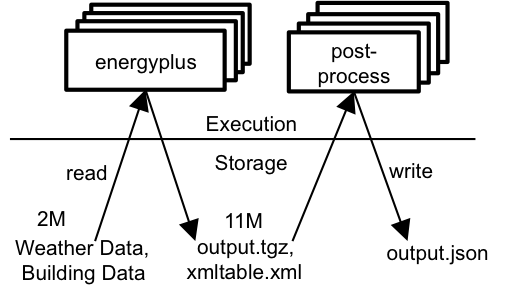
\includegraphics[width=2in]{figures/eplus.png}
%\label{fig_snap}
\caption{EnergyPlus application and its interaction with storage systems. 
\label{fig_eplus}
}
\end{center}
\end{figure}

\begin{figure}[htb]
\begin{center}
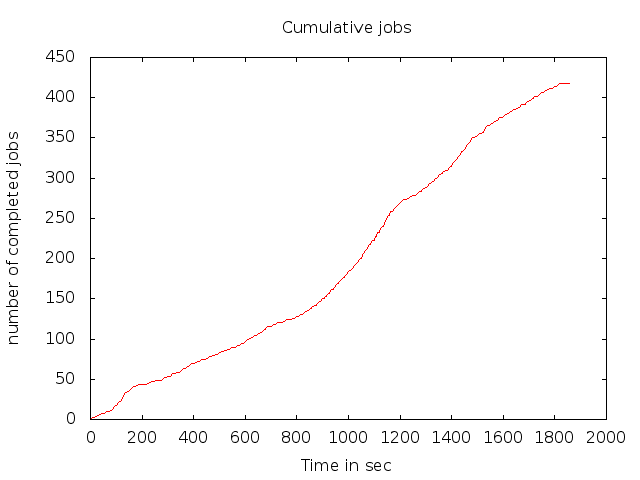
\includegraphics[width=\linewidth]{plots/eplus_40i_80c.png}
%\label{fig_snap}
\caption{EnergyPlus application cumulative task execution plot with
Swift/K data staging; A total of 420 tasks run on 40 cloud instances. 
\label{fig_eplus_k}
}
\end{center}
\end{figure}

\begin{figure}[htb]
\begin{center}
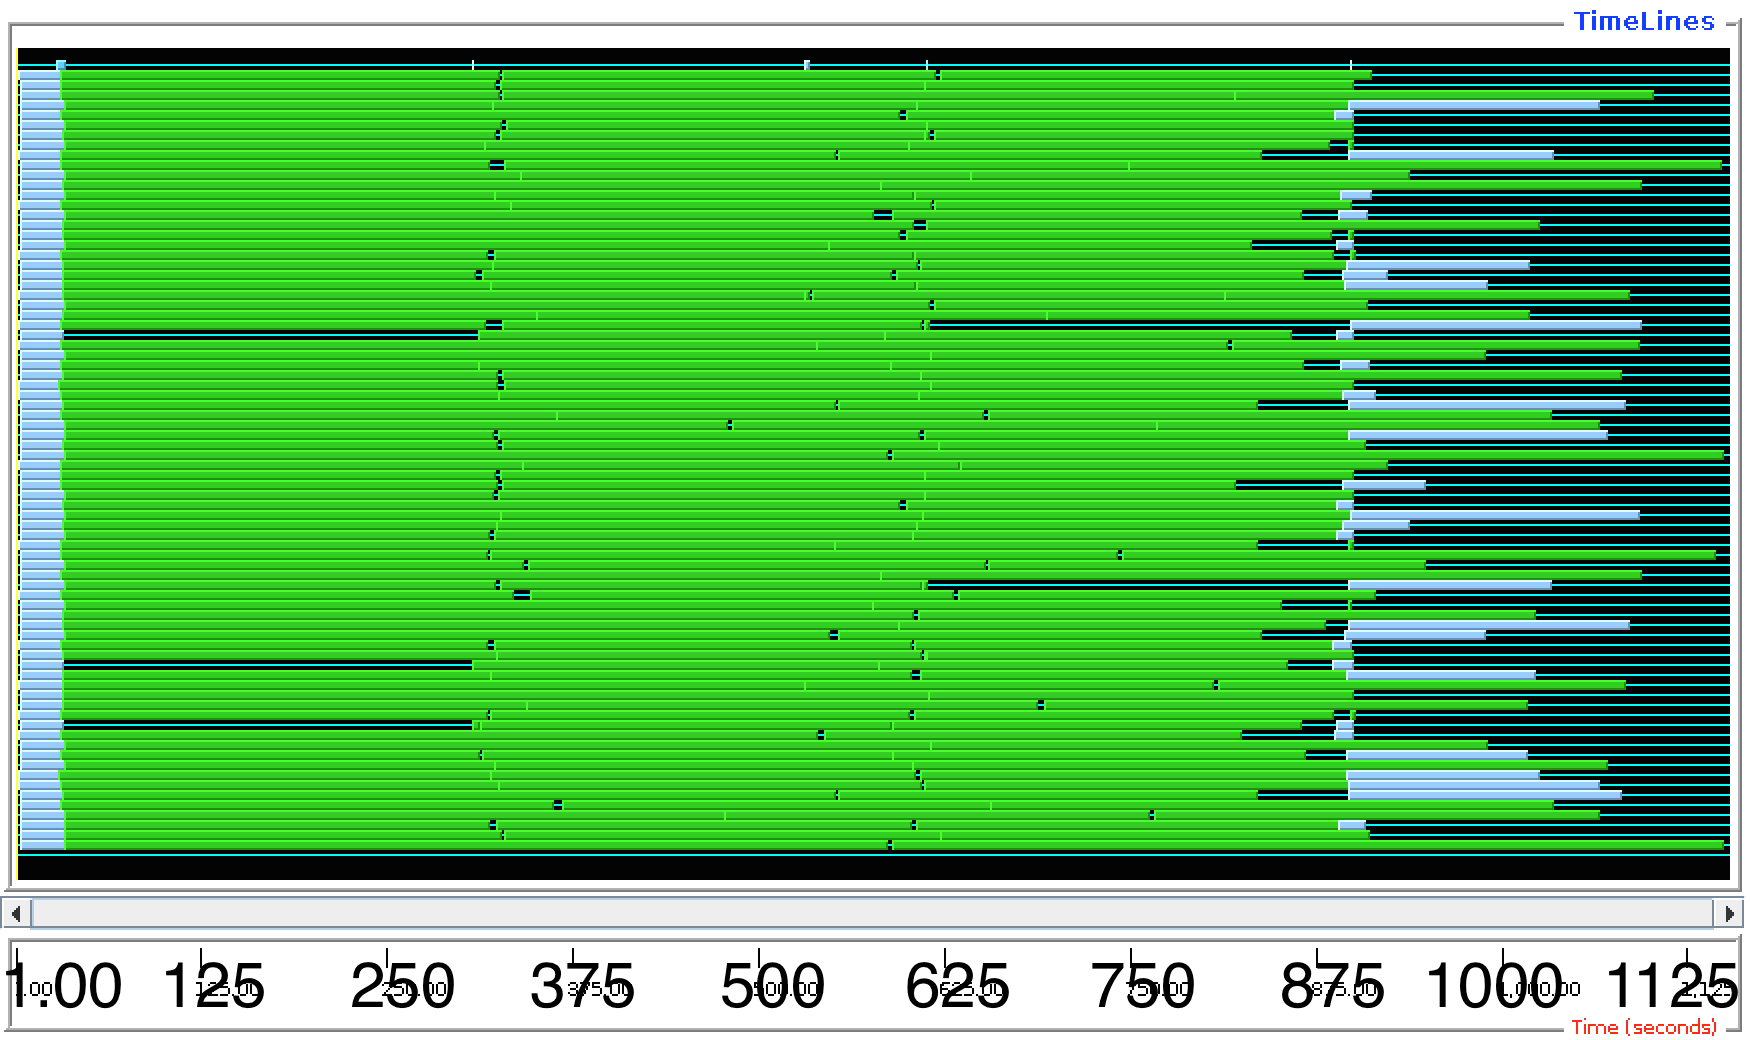
\includegraphics[width=\linewidth]{plots/eplus_timeline_40i_80c.png}
%\label{fig_snap}
\caption{The Energy plus application execution trace with Swift/T and Mosastore
as data staging platform; A total of 420 tasks run on 40 cloud instances.
The light blue bars indicate worker-coordination wait, green bars
indicate the executions.
\label{fig_eplus_t}
}
\end{center}
\end{figure}

\section{Evaluation} \label{sec:appresults}
In this section, we discuss the results and an evaluation of our study.
Figure~\ref{fig:makespan} shows the power grid application end-to-end
makespan times for an increasing number of instances on global locations of EC2
instances starting from 20 to 120 with different virtual storage systems. 

We use the local disk writes as a baseline for these experiments. While raw
local writes are faster on the local file systems, the
results are available only to the nodes where the computation was done. In
order to gather results at the end of the computation, an additional expensive
stage out operation is required which is eliminated by virtue of the storage
systems.

The general trend we see from the plot in figure~\ref{fig:makespan} is a sharp
improvement in execution performance in the initial increments of nodes from 20
to 60. We notice a knee in the performance curve at node count 60 because the
allocation goes beyond the United States region after this point. A steady
improvement is observed after this point followed by no significant
improvements despite adding nodes as indicated by a near-plateau between 80 and
120 nodes especially in the case of Amazon S3. This behavior is expected
because as the number of nodes increases the amount of communication to remote
instances from a centrally located S3 servers is added on top of application
communications. A general trend of steady performance (flat curve) after 60
nodes is expected for other storage systems because of the remote location of
regions beyond 60 nodes drawn from the EU and Asian data centers.

\begin{figure}[htb]
\begin{center}
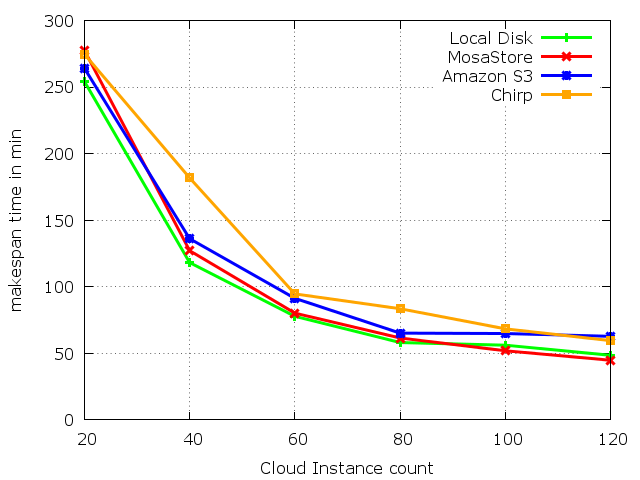
\includegraphics[width=\linewidth]{plots/makespan.png}
\caption{Application makespan times with results written to local disk and
virtual storage systems on an increasing number of cloud instances.
\label{fig:makespan}
}
\end{center}
\end{figure}

Figures~\ref{fig_blast_k} and~\ref{fig_eplus_k} show cumulative task completion
plots for the Blast and EnergyPlus applications respectively, generated from
the Swift/K execution log. The executions are carried out via Swift/K coasters
setup and using an explicit staging mechanism. Figures~\ref{fig_blast_t}
and~\ref{fig_eplus_t} respectively show application completion results via
Swift/T with MosaStore as storage solution in an alternative task trace
representation obtained via MPE~\cite{mpe}.

The difference between the Swift/T and Swift/K executions is data staging. While
Swift/K performs explicit on-demand data movement, Swift/T assumes a shared
data access across executions. In a distributed cloud environment this is made
possible by virtue of the storage systems. Clearly, Swift/T storage system
driven applications (Figs.~\ref{fig_blast_t} and~\ref{fig_eplus_t}) perform
better than Swift/K explicit staging applications
(Figs.~\ref{fig_blast_k} and~\ref{fig_eplus_k}).

\section{Related Work} \label{sec:related}
In this section, we discuss projects related to storage, computation, and
execution management in the cloud environments. 
%We focus on the
%following capabilities and system attributes:
%
%\begin{enumerate}
%
% \item \label{itm:one} Utility of storage solutions: space aggregation,
%     transparent access, performance, durability, locality, extensibility,
%     configurability and ease of setup.
%
% \item \label{itm:two} Computational models in the cloud: programmability, task
%     granularities, flexibility, and compatibility with storage systems.
%    
% \item Usability: Improvement in overall usability of cloud environments with respect to solutions mentioned in~\ref{itm:one}
% and~\ref{itm:two}.
%
%\end{enumerate}
%

The cloud model of computing presents several distinct data management
techniques. Work described in~\cite{cloud-dataintensive} addresses the need
for data oriented services specific to cloud environments such as content
specific access and security. Work described in ~\cite{rebalance} presents
algorithms to augment the load balancing among file blocks on distributed
storage systems such as HDFS.

Other projects have used clouds to extend high-end computing, for example a
federated computing in the CometCloud project~\cite{cometcloud_web}. CometCloud
offers a layered suite of services for managing multiple applications (via
workflow, Master/Worker, and MapReduce services) on aggregated computational
platforms (via accessibility, overlay and communication services).  Benchmarks
similar to ours have been documented in recent cloud
evaluation~\cite{cloudefficacy} in a computational context.

A study by one of the authors of current work raised doubts about S3's
appropriateness as a live storage system for distributed
applications~\cite{s3-viable}, citing a lack of support for flexible access
control and concerns about high-performance data access. However, the same
study cite several features such as data durability, high-availability, and
ease of access via POSIX (achievable on top of FUSE) or other APIs (e.g., the
REST API) that can make S3 an appealing storage solution for scientific
applications. Our work back the findings with application performance results
as evidence and lays further motivation for usage of aggegated, node-local
storage systems in the clouds.

%Variants of Hadoop have been implemented for scientific
%applications such as Marissa~\cite{marissa} addressing HDFS
%accessibility and performance for applications that are not ported for
%Java. Our approach differs from Hadoop in that we use the highly general
%Swift programming model to generate and distribute tasks, while using
%Swift-automated staging or ad hoc data access techniques depending on
%the underlying storage system.  As shown in our application results,
%this provides high levels of generality and flexibility with respect
%to the workflow pattern, application domain, and underlying
%infrastructure. 

\section{Conclusions}\label{sec:concl}
We evaluate two representative storage systems each from scientific and
commercial domain in the cloud. With an availability of local ephemeral storage
and remote object storage in the form of S3, data handling in clouds poses
intriguing challenges.  We attempt to address these challenges by understanding
the network characteristics of a commercial cloud implementation and setting up
the cloud with Swift orchestrated computations over storage systems. We
benchmark our approach with basic read and write patterns commonly observed in
scientific applications. With the current state of the art of this work, we
draw the following main conclusions:

\begin{itemize}
  \item Globally implemented clouds rely heavily on internet backbone resulting in a non-uniform and variable network characteristics which application deployments must take into account. Storage solutions can mitigate resulting variabilities to some extent by techniques such as caching, replication and prediction.
  \item Applications with small to medium immediate storage requirements can be run effectively by aggregating the cloud node-local space with the help of storage solutions. These solutions almost always perform better compared to the dedicated object store provided by clouds such as S3 by Amazon.
  \item Storage solutions such as S3 are nonetheless important for large-scale data handling and archival purposes.
  \item Depending upon the application requirements, Swift can handle both implicit and explicit data motions in the cloud.
\end{itemize}

For data motion during an application execution, we study two approaches:
explicit workflow engine staged data movement and implicit data movement via
coupling the virtual storage systems with workflow systems. We chose HDFS for
its popularity, MosaStore for its ability to offer a shared POSIX-compatible
and at the same time support optimizations for workflow applications, and
Chirp/Parrot for its ease of deployment. From the results obtained from
benchmarking and actual application studies with different cloud configurations
(local, single zone, and global) we were able to understand the effectiveness
of storage systems. We show how real-world application data can be handled in
the cloud by using storage systems. In particular, our experiments shed light
on utility and performance of storage systems as an alternative to the de
facto S3 storage offered by Amazon. 

\section*{Acknowledgments}
This work was partially supported by the U.S. Department of Energy, under
Contract No. DE-AC02-06CH11357. We thank Gail Pieper for proofreading help. We
thank Amazon for AWS Amazon research grant award. Some work by DSK was supported by
the National Science Foundation, while working at the Foundation. Any opinion,
finding, and conclusions or recommendations expressed in this material are
those of the authors and do not necessarily reflect the views of the National
Science Foundation. 

\bibliographystyle{IEEEtran}
\bibliography{ref}
\end{document}

